\documentclass[twocolumn, 11pt]{article}%
\usepackage{amsmath, amssymb, esint, gensymb, hyperref, mathtools}
\usepackage{graphicx, cuted, geometry, float, scalerel, xcolor, chemfig}

\newcommand\sbullet[1][.5]{\mathbin{\ThisStyle{\vcenter{\hbox{%
  \scalebox{#1}{$\SavedStyle\bullet$}}}}}%
}

\geometry{
    a4paper,
    total={170mm,260mm},
}

\begin{document}

\begin{strip}
  \vspace*{\dimexpr-\stripsep}
  \begin{center}
      \Large\textbf{FISIKA 2}\\
      \large{Pertemuan 1 - Minggu 4 (852724)}\\
      \large{\today}
   \end{center}
\end{strip}

\section{Kapasitor}
    \begin{center}
        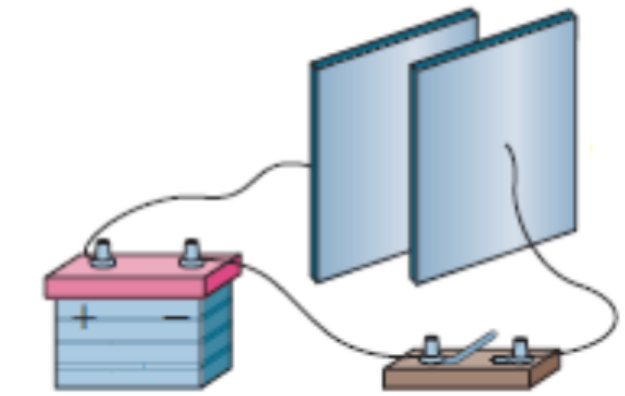
\includegraphics[width=120px]{2.png}
    \end{center}
    Kapasitor adalah perangkat yang dapat menyimpan energi dalam medan listrik. Secara umum kapasitor terbentuk dari dua buah konduktor yang diberi muatan (sama besar tapi berbeda jenis) dan terpisah oleh suatu bahan isolator (dinamakan bahan dielektrik).

    \begin{center}
        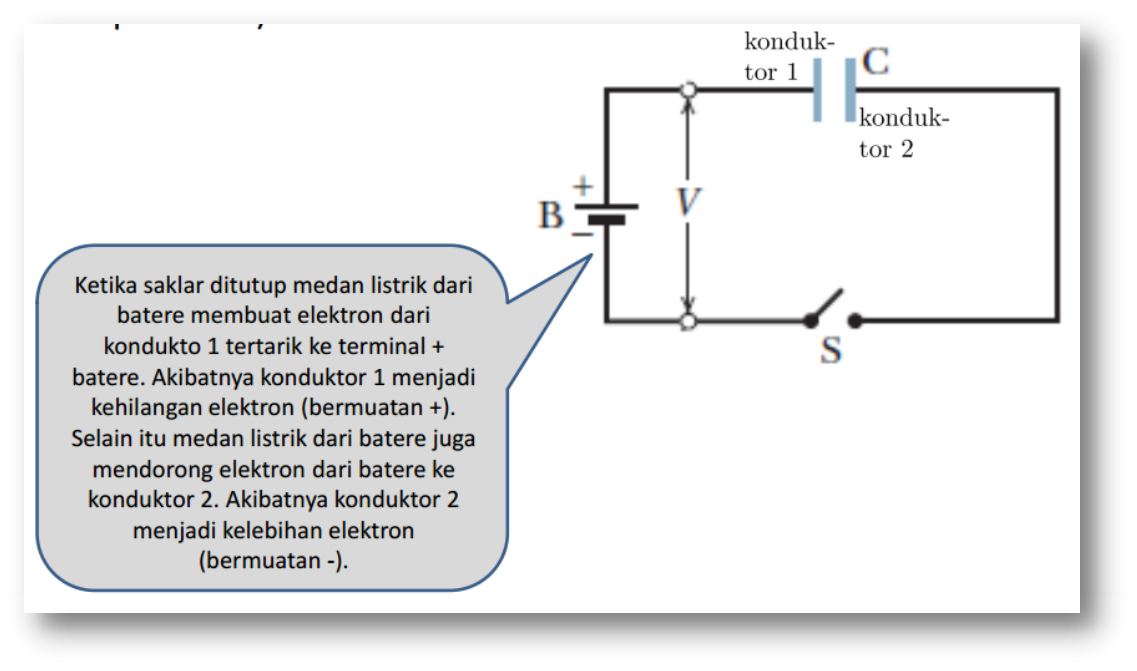
\includegraphics[width=220px]{3.png}
    \end{center}

    Proses pemberian muatan (pengisian) kapasitor dilakukan dengan menghubungkan kapasitor dengan sumber tegangan (beda potensial) tertentu.

    \subsection{Kapasitas/Kapasitansi suatu Kapasitor}%
    Muatan yang tersimpan dalam suatu sistem kapasitor sebanding dengan besar beda potensial yang diberikan $Q\propto\Delta V$.

    Faktor kesebandingan antara muatan yang tersimpan dengan beda potensial yang diberikan dinamakan kapasitansi, yang menyatakan kemampuan kapasitor untuk menyimpan muatan, disimbolkan dengan $C$.
    \[Q=C\Delta V\]
    Satuan kapasitansi biasanya bergantung pada bentuk, ukuran posisi relatif antar konduktor bedakan.

    Untuk menentukan kapasitansi suatu kapasitor:
    \begin{itemize}
        \item Tentukan medan listrik akibat konduktor yang bermuatan (anggap masing-masing konduktor bermuatan sebesar $Q$). Dapat diperoleh menggunakan hukum Gauss ataupun hukum Coulomb.
        \item Tentukan beda potensial antara kedua konduktor.
        \item Tentukan kapasitansi sistem kapasitor tersebut dengan mengingat bahwa kapasitansi merupakan perbandingan antara muatan dengan beda potensial yang terjadi.
    \end{itemize}

    \begin{center}
        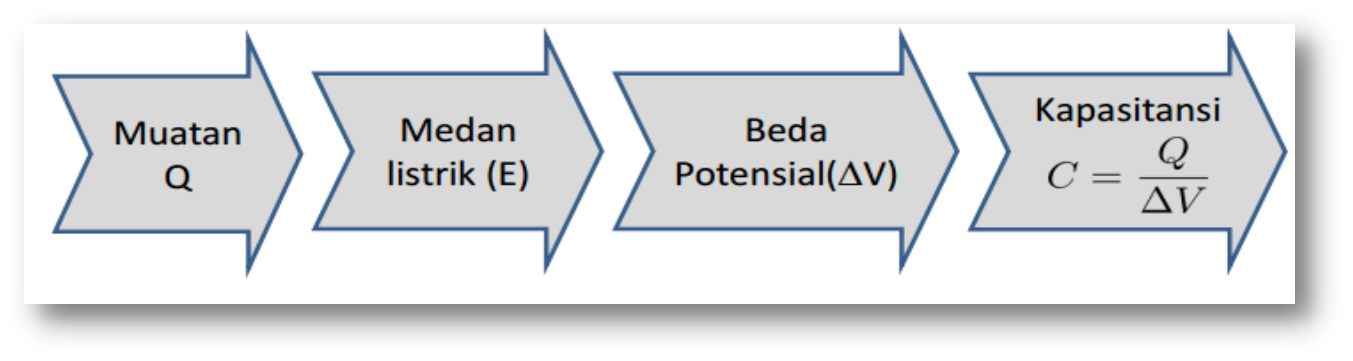
\includegraphics[width=200px]{1.png}
    \end{center}

    \subsection{Bentuk-bentuk Kapasitor}%
    \subsubsection{Kapasitor Keping Sejajar}%
    Medan listrik dekat permukaan oleh lempeng yang sangat besar, bermuatan $Q$ dan luas permukaan $A$.
    \begin{center}
        $\displaystyle E=\frac{\sigma}{2\epsilon_0}$ dengan $\displaystyle \sigma = \frac{Q}A$
    \end{center}

    Medan listrik diantara dua keping lempeng adalah
    \begin{center}
        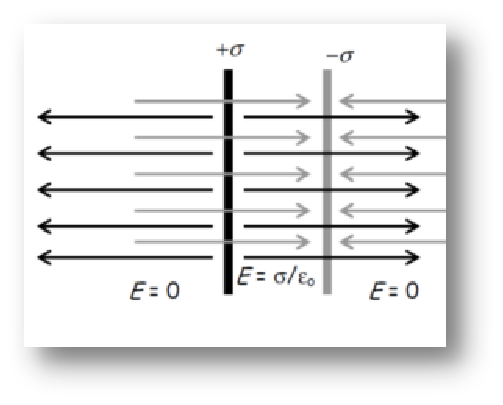
\includegraphics[width=150px]{4.png}
    \end{center}
    \[2E=\frac{\sigma}{\epsilon_0}=\frac{Q}{A\epsilon_0} \]

    Jadi, beda potesial diantara dua keping ialah
    \begin{align*}
        V_b-v_a&=-\int\limits_a^b E\ ds\\
        \Delta V&=\int\limits_0^d E\ ds=Ed
    \end{align*}

    Maka,
    \[C=\frac{Q}{\Delta V}=\frac{A\epsilon_0 E}{Ed}=\frac{\epsilon_0A}d \]

    \subsubsection{Kapasitansi Kapasitor Silinder}%
    \begin{center}
        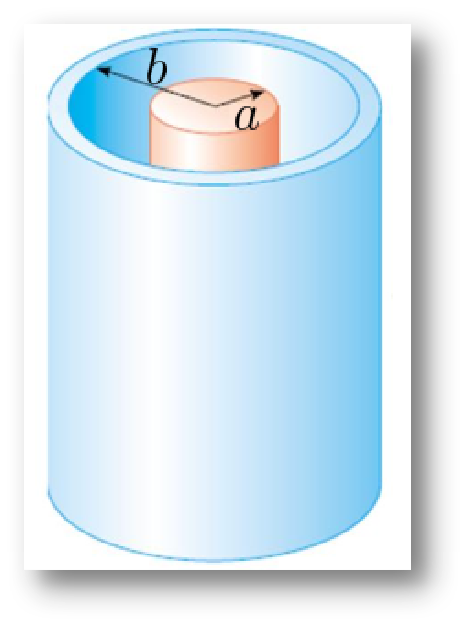
\includegraphics[width=80px]{5.png}
        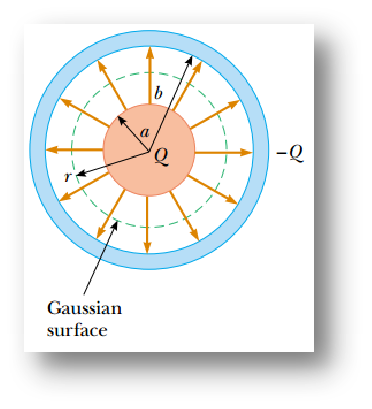
\includegraphics[width=100px]{6.png}
    \end{center}

    Medan listrik pada ruang antar kedua konduktor (jarak $r$ dari konduktor dalam)
    \[E=\frac{Q}{2\pi\epsilon_0Lr} \]

    Beda potensial antara kedua konduktor
    \[\Delta V=\frac{Q}{2\pi\epsilon_0L} \ln\left(\frac{b}a \right) \]

    Kapasitansinya adalah
    \[C=\frac{Q}{\Delta V}=\frac{2\pi\epsilon_0L}{\ln\left(\frac{b}a \right)} \]

    \subsubsection{Kapasitansi Kapasitor Bola}%
    \begin{center}
        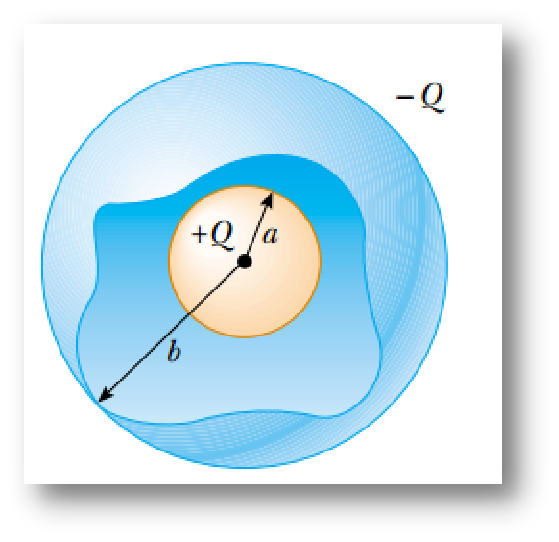
\includegraphics[width=100px]{7.png}
    \end{center}

    Medan listrik pada ruang antara kedua konduktor
    \[E=\frac{Q}{4\pi\epsilon_0 r^2} \]

    Beda potensial antara kedua konduktor
    \begin{align*}
        V_b-V_a &=-\int\limits_a^b E\ dr\\
        \Delta V&=-\int\limits_a^b \frac{Q}{4\pi\epsilon_0 r^2}\ dr\\
        \Delta V&=\frac{Q}{4\pi\epsilon_0} \left(\frac1b - \frac1a \right)\\
        \Delta V&= \frac{Q}{4\pi\epsilon_0} \left(\frac{b-a}{ab}\right)
    \end{align*}

    Kapasitansinya
    \[C=\frac{Q}{\Delta V}=\frac{4\pi\epsilon_0(ab)}{(b-a)} \]

    \subsection{Susunan Kapasitor}%
    \begin{center}
        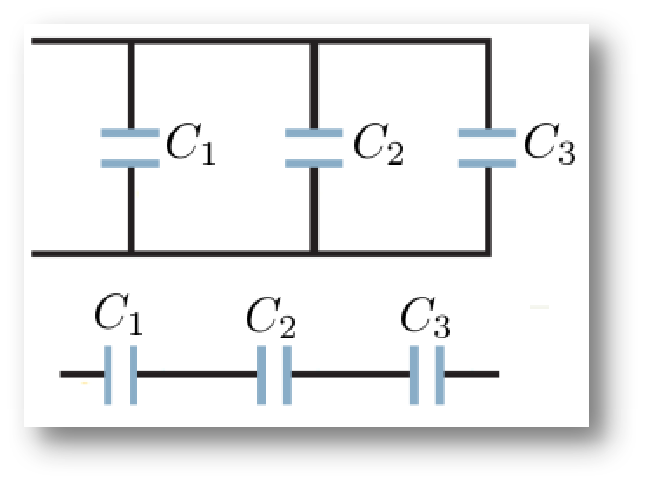
\includegraphics[width=150px]{8.png}
    \end{center}
    Dalam rangkaian listrik dua atau lebih kapasitor dikombinasikan. Susunan ini memberikan suatu “kapasitor baru” dengan nilai kapasitansi yang juga baru, diistilahkan sebagai kapasitansi ekivalen atau kapasitansi pengganti atau kapasitansi total susunan kapasitor.

    Ada dua macam kombinasi dasar kapasitor: \textbf{Seri dan Paralel}.
    Kombinasi lainnya yang lebih rumit dapat dipandang sebagai kombinasi dari seri dan paralel.

    \subsubsection{Paralel}%
    \textbf{Tengangannya (beda potensial) TETAP}
    \begin{center}
        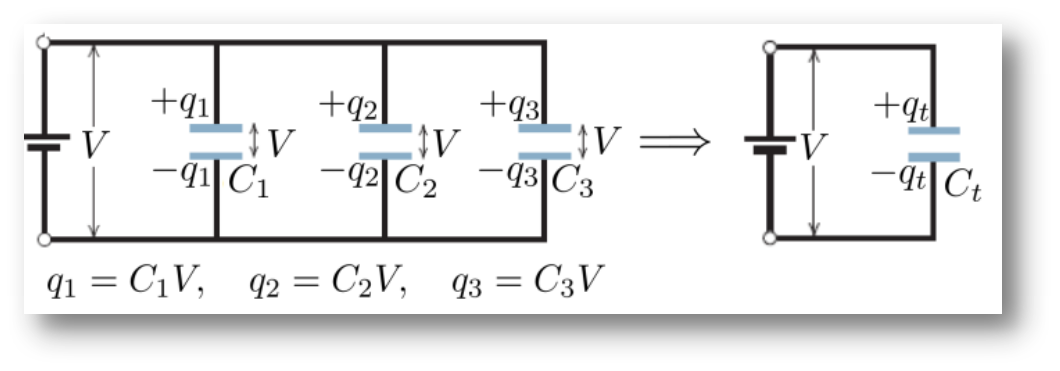
\includegraphics[width=220px]{9.png}
    \end{center}
    Muatannya totalnya adalah
    \[q_{\text{total}}=q_1+q_2+q_3 \]

    Dan kapasitansi totalnya adalah
    \[C_{\text{pengganti}}=\sum^N_{i-1} C_i \]

    \subsubsection{Seri}%
    Muatan tiap-tiap kapasitor \textbf{SAMA BESAR} 
    \begin{center}
        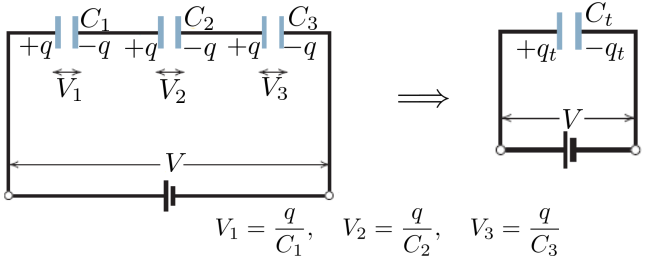
\includegraphics[width=200px]{10.png}
    \end{center}

    Tegangannya adalah
    \[V_{\text{total}}=V_1+V_2+V_3\]

    dan kapasitansi totalnya (kapasitansi penggantinya) adalah
    \[\frac1{C_{\text{pengganti}}}=\sum^N_{i=1} \frac1{C_i} \]

    \subsection{Energi Dalam Kapasitor}%
    Selama proses pengisian kapasitor, dapat dipandang bahwa muatan dipindahkan dari salah satu konduktor ke konduktor lainnya. Jika muatan sebesar $q$ dipindahkan dari suatu tempat ke tempat lain yang mempunyai beda potensial $V$, maka energi potensial muatan tersebut bertambah sebesar $qV$

    Ini berarti untuk mengisi kapasitor diperlukan sejumlah usaha (energi). Energi ini kemudian disimpan dalam bentuk energi potensial muatan yang berpindah. Energi yang diperlukan untuk memindahkan muatan sebesar dq pada beda potensial $V$ adalah :
    \[dU=V\ dq\]

    Energi yang dibutuhkan untuk mengisikan muatan sebesar $Q$ (dari keadaan kosong) adalah
    \begin{align*}
        U&=\int\limits_0^Q dU=\int\limits_0^Q V\ dq=\int\limits_0^Q \left(\frac{q}{C}\right)\ dq\\
         &=\frac{Q^2}{2C}
    \end{align*}

    Energi yang tersimpan dalam kapasitor yang bermuatan $Q$ dengan kapasitansi $C$ dan beda potensial $V$
    \[U=\frac{Q^2}{2C}=\frac12 QV=\frac12CV^2 \]

    Energi yang tersimpan dalam kapasitor bisa dicontohkan dengan bentuk penyimpanan energi dalam medan listrik, misalnya untuk kapasitor keping sejajar

    \begin{align*}
        U&=\frac12 CV^2\\
         &=\frac12 \left(\frac{\epsilon_0 A}d\right)(Ed)^2\\
         &=\frac12(\epsilon_0Ad)E^2
    \end{align*}

    Sedangkan Rapat energinya ialah (energi per satuan volume)
    \[u=\frac{U}{Volume}=\frac12 (\epsilon_0Ad) E^2 \]

    Bentuk yang sama juga dapat diperoleh untuk kapasitor lainnya (tidak cuma kapasitor keping sejajar). Coba turunkan rumusnya sendiri

    \subsection{Bahan Dielektrik}%
    Ruang antar konduktor pada kapasitor biasanya berisi bahan isolator (non-conducting) yang disebut sebagai bahan dielekrik, misalnya kertas, mika, dll.

    Eksperimen yang dilakukan Faraday menunjukkan bahwa adanya bahan dielektrik menyebabkan \textbf{kapasitansi suatu} kapasitor bertambah. Adanya bahan dielektrik menyebabkan \textbf{medan listrik} dalam ruang di antara konduktor pada kapasitor menjadi berkurang.

    Karakteristik suatu bahan dielektrik dinyatakan dengan besaran yang disebut konstanta dielektrik ($K$)

    Bahan dielektrik memiliki dua jenis, yaitu polar dan non-polar

    \subsubsection{Polar}%
    Bahan dielektrik polar (polar dielectrics), mempunyai momen dipole listrik yang permanen, misalnya air
    \begin{center}
        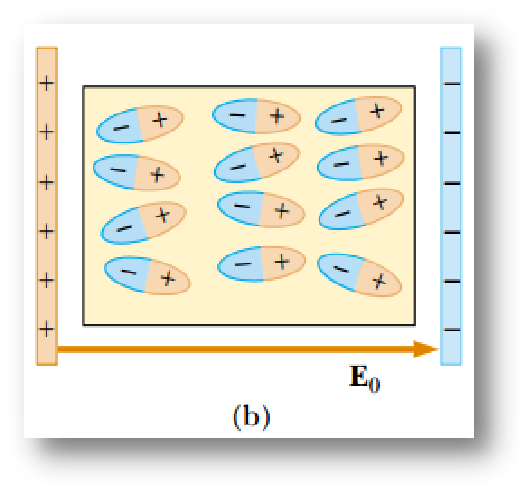
\includegraphics[width=100px]{11.png}
    \end{center}

    \subsubsection{Non-polar}%
    Bahan dielektrik nonpolar (nonpolar dielectrics), momen dipole listrik muncul akibat berada dalam medan listrik. Molekul bahan dielektrik akan terpengaruh medan listrik.
    \begin{center}
        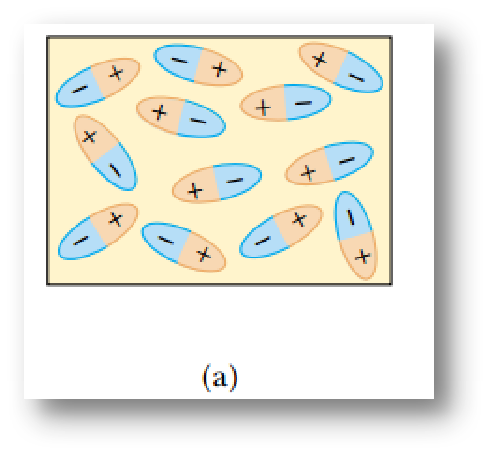
\includegraphics[width=100px]{12.png}
    \end{center}
    
    \subsubsection{Perhitungan Bahan Dielektrik}%
    \begin{center}
        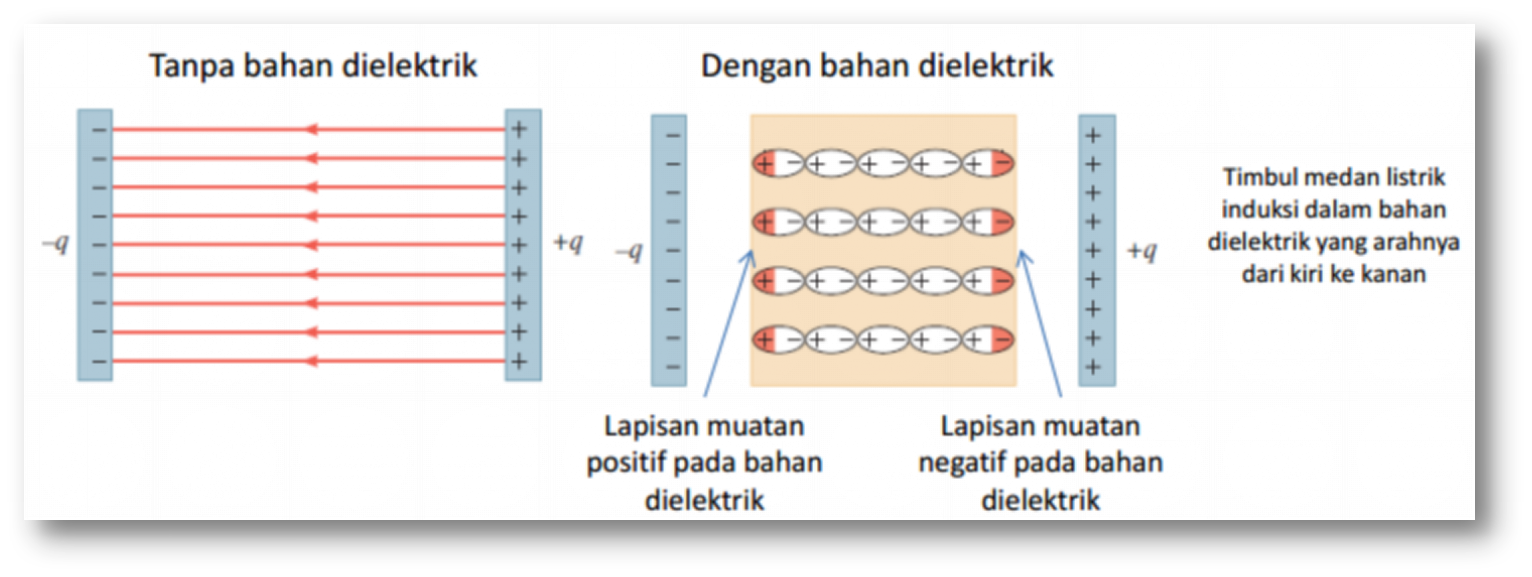
\includegraphics[width=220px]{13.png}
    \end{center}

    Medan listrik total dalam bahan adalah
    \[\vec E=\vec E_0 + \vec E_{ind} \]

    \begin{center}
        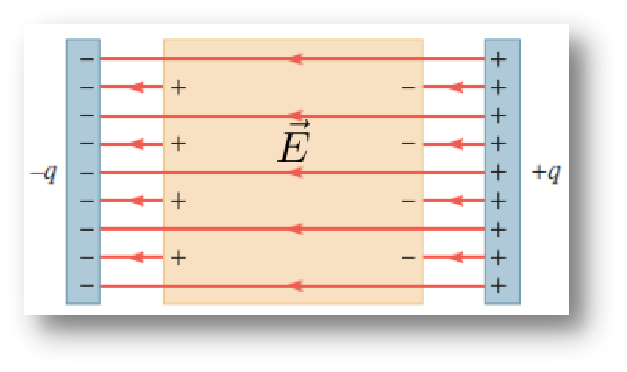
\includegraphics[width=200px]{14.png}
    \end{center}

    $\vec E_{ind}$ arahnya berlawanan dengan $\vec E_0$. Sehingga\\
    \[ |\vec E| < |\vec E_0|\]
    
    Dapat dinyatakan bahwa $E\propto E_0$, atau
    \[ E_0=KE \]

    dimana $K$ adalah konstanta dielektrik, yaitu karakteristik bahan dielektrik
    \[K>1\ \Rightarrow\ E_0 > E \]

    Karena medan listrik berkurang, maka beda potensial juga berkurang (untuk jumlah muatan yang tetap)
    \[V=\frac{V_0}{K} \]

    Sehingga kapasitansi kapasitor dengan dielektrik adalah
    \[C=\frac{Q_0}{V}=\frac{Q_0}{V_0/K}=K\frac{Q_0}{V_0}=KC_0 \]

    Karena $K>1$ maka $C>C_0$

    \subsubsection{Lain-lain}%
    Konstanta dielektrik terkait besaran permitivitas bahan $\epsilon=K\epsilon_0$. Dengan demikian konstanta dielektrik dapat juga disebut sebagai permitivitas relatif suatu bahan (relatif terhadap medium vakum (free space).

    Dengan adanya bahan dielektrik pada kapasitor maka ada nilai maksimum beda potensial yang dapat diberikan antara keping kapasitor yaitu
    \[\Delta V_{max}\]

    yang disebut juga sebagai \textit{breakdown potential}.

    Hal ini terkait dengan karakteristik yang disebut \textit{dielectric strength}, yang menyatakan besar maksimum medan listrik yang masih dapat diterima oleh suatu bahan dielektrik.
    
\end{document}
